\documentclass[main.tex]{subfiles}
\begin{document}

\section{Deterministic Soft CCP}\label{sec:detSCCP}
This section introduces our (meta-)language.
We fix a set of variables $V$, ranged over by $x$, $y$, $\ldots$ , and 
an invertible CLIM $\mathbb S = \langle {\mathcal C}, \leq, \otimes\rangle$, which is 
cylindric over $V$ and whose compact elements
are ranged over by $c$, $d$, $\ldots$.

\begin{definition}[Agents]%
The set $\mathcal{A}$ of all agents, %which is
parametric with respect to a set $\mathcal{P}$ of (unary) procedure declarations $p(x)$,
is given by the following grammar
\[ A \Coloneqq \: \: \mathit{\ostop} \mid \textit{\tell}(c)  \mid \textit{\ask}(c) \rightarrow A \mid A \parallel A \mid \exists_x A \mid %Z \mid \mu_Z A
p(x).\]  
\end{definition}

We denote by $fv(A)$ the set of free variables of an agent, defined in the expected way 
by structural induction, assuming that $fv(\tell(c)) = sv(c)$ and
 $fv(\ask(c) \rightarrow A) = sv(c) \cup fv(A)$.
 %
 In the following, we restrict our attention to 
 procedure declarations $p(x) = A$ such that $fv(A) = \{x\}$.

%
%
%%Given a soft constraint system $S_C=\langle \C, \otimes,\bot,\top ,
%%\exists_x, d_{xy}\rangle$ as defined in
%%Section~\ref{sec:softconstraints}, the syntax
%%of  deterministic \SCCP agents is defined as
%
%
%\def\odivv{\; {\ominus\hspace{-4pt} \div} \;}
%\def\odivvv{\; {\ominus\hspace{-6pt} \div} \;}
%\begin{table}
%%\footnotesize
%\begin{center}
%%P \Coloneqq \: \: F.A \; \; \; \; \; \; \; \;
%%F \Coloneqq \: \: p(\hat{x})::A \mid F.F \; \; \; \; \; \; \; \;
%$A \Coloneqq \: \: \mathit{\ostop} \mid \textit{\tell}(c)  \mid \textit{\ask}(c) \rightarrow A \mid A \parallel A \mid \exists_x A \mid %Z \mid \mu_Z A$
%p(x)$
%\end{center}
%%\normalsize
%\caption{The syntax of deterministic soft CCP}
%\label{syntax}
%\end{table}
%
%In Tab.~\ref{syntax} we recall the deterministic fragment of soft CCP,
%with respect to the standard proposal, we replaced the procedure call with the
%simpler to handle recursion operator $\mu_Z$.
%%\marginpar{A che servono F e P?}
%%
%Let $\mathcal{A}$ be the set of all agents, which is
%parametric with respect to a set $\mathcal{P}$ of (unary) procedure declarations 
%$p(x) = A$ such that $fv(A) = \{x\}.$\footnote{The set of free variables of an agent is defined in the
 %expected way by structural induction, assuming that $fv(\tell(c)) = sv(c)$ and $fv(\ask(c) 
 %\rightarrow A) = sv(c) \cup fv(A)$.}
%
%$\mathcal{P}$ is the class of programs, $\mathcal{F}$ is the class of sequences of procedure
%declarations,
%$\mathcal{A}$ is the set of agents and
%$\mathcal{Z} = \{Z, Z_1, Z_2 \ldots\}$ is the set of recursion variables, 
%$c \in \C^\otimes$ with $sv(c) \in V$.
%
%, and $\hat{x}$ is a tuple of variables in $Var$ passed in a procedure call.
%
%In $p(\hat{x}) :: A$ we assume that the variables in
%$\mathit{vars}(A)$, i.e. the set of variables occurring either as parameters of procedure calls or belonging
%to the support of
%the constraints in agent $A$, also occur
%among $\hat{x}$.
%\footnote{Note that, with respect to the standard proposals, we require only for the
%$\textit{ask}$ operator to have a compact constraint, while the $\textit{tell}$ ranges over all constraints.
%Intuitively, we allow to require to the store the removal of certain constraint, while compactness allow
%for obtaining a simpler relation when checking the entailment of a constraint.}

We now move to consider the reduction semantics of our language.

\begin{definition}[Substitutions]
Let $x$, $y$ be variables in $V$. 
The substitution $[^y/_x]: \mathcal{A} \rarrow \mathcal{A}$ is a function 
on agents defined by structural induction as 

\begin{itemize}
\item $\0 [^y/_x] = \0$
\item $\tell(c) [^y/_x] = \tell(c [^y/_x])$
\item $p(w) [^y/_x] = \begin{cases} p(y) & \text{if $w = x$}\\
                                                        p(w) & \text{otherwise}
                                 \end{cases}$
\item $(\ask(c) \rightarrow A) [^y/_x] = \ask(c[^y/_x]) \rightarrow A [^y/_x]$
\item $(\exists_w A) [^y/_x]  = \begin{cases} \exists_w A & \text{if $w = x$}\\
                                                                      \exists_z (A[^z/_y][^y/_x]) & \text{for $z$ fresh if $w = y$}\\
                                                                      \exists_w (A[^y/_x]) & \text{otherwise}
                                 \end{cases}$
\item $(A_1 \parallel A_2) [^y/_x]  = (A_1 [^y/_x] \parallel A_2 [^y/_x] )$
\end{itemize}
\end{definition}

The substitution on compact elements is the one given in Definition~\ref{def:sub}: thanks to Lemma~\ref{lemmaSubs0}, 
the choice of the intermediate variable is immaterial.
% NO
% $A[^y/_z][^z/_x] = A[^y/_x]$, since each syntactical substitution in $A$ involves all the variables with the same name.



\begin{definition}[Reductions]\label{def:reductions}
Let $\Gamma = {\mathcal A} \times \C^\otimes$ be the set of \emph{configurations}.
The \emph{direct reduction semantics} for SCCP is the pair 
$\langle \Gamma,  \mapsto \rangle$
such that $\mapsto \, \, \subseteq \, \,\Gamma \times   \Gamma$ is the family 
 of binary relations indexed over sets of variables,
%$2^V$,
%between them, 
i.e., $\mapsto = \bigcup_{\Delta \subseteq V} \mapsto_\Delta$ and 
$\mapsto_\Delta \, \, \subseteq \, \,\Gamma \times \Gamma$, obtained by the rules in 
Table~\ref{fig:operational}.

The \emph{reduction semantics} for SCCP is the pair 
$\langle \Gamma,  \rightarrow \rangle$
such that $\rightarrow \, \, \subseteq \, \,\Gamma \times   \Gamma$ is the family 
 of binary relations indexed over sets of variables,
%$2^V$,
%between them, 
i.e., $\rightarrow = \bigcup_{\Delta \subseteq V} \rrarrow_\Delta$ and 
$\rrarrow_\Delta \, \, \subseteq \, \,\Gamma \times \Gamma$, obtained by the rules in 
Table~\ref{fig:operational} and Table~\ref{fig:operational2}.
\end{definition}

%\vspace{-.25cm}
\def\odiv{\; {\ominus\hspace{-6pt} \div} \;}
\def\odivvv{\; {\ominus\hspace{-6pt} \div} \;}

\begin{table}  %\hfil5
  %\scalebox{0.9}{
   \begin{center}
   \begin{tabular}{llll} 
   %
   \mbox{\bf A1}& $\frac{\displaystyle sv(\sigma) \cup sv(c) \subseteq \Delta } {\displaystyle \langle \hbox{\tell}(c), \sigma \rangle \mapsto_\Delta  \langle \hbox{\ostop},
                                               \sigma \otimes c\rangle}$
   \ \ \ & \bf{Tell}&
  \\ 
  &\mbox{   }&\mbox{   } &\mbox{   }
  \\
  \mbox{\bf A2}& $\frac {\displaystyle sv(\sigma) \cup sv(c) \cup fv(A) \subseteq \Delta \wedge c \leq \sigma}{\displaystyle
  	\begin{array}{l} \langle \hbox{\ask}(c) \rightarrow A, \sigma \rangle \mapsto_\Delta \langle A, \sigma \rangle   	\end{array}}$
    \ \ \ & \bf{Ask}&
    \\
    &\mbox{   }&\mbox{   }&
    \\
  \mbox{\bf A3}& $\frac {\displaystyle sv(\sigma) \cup \{y\} \subseteq \Delta \wedge \displaystyle p(x) = A \in  \mathcal{P} }
  {\displaystyle\langle p(y),\sigma\rangle \mapsto_\Delta \langle  A[^y/_x], \sigma\rangle}$ 
  &\bf{Rec}&
    \\
   &\mbox{   }&\mbox{   }&
  \\
    \mbox{\bf A4}& $\frac {\displaystyle sv(\sigma) \cup fv(\exists_x A) \subseteq \Delta 
    \wedge w \not \in \Delta }
    {\displaystyle\langle \exists_x A,\sigma\rangle \mapsto_\Delta \langle A[^w/_x], \sigma\rangle}$
    &\bf{Hide}&
  \end{tabular}
  \end{center}
\caption{Axioms of the reduction semantics for SCCP.}
\label{fig:operational}
\end{table}

\begin{table}  %\hfil5
  %\scalebox{0.9}{
   \begin{center}
   \begin{tabular}{llll} 
   %
  \mbox{\bf R1}& $\frac {\displaystyle \langle A,\sigma \rangle \rrarrow_\Delta \langle A', \sigma' \rangle
  \wedge fv(B) \subseteq \Delta} 
  {\displaystyle \begin{array}{l}
                          \langle A\parallel B, \sigma \rangle \rrarrow_\Delta \langle A'\parallel B, \sigma' \rangle
                          \end{array}}$ 
    & \bf{Par1}&
  \\
  & \mbox{   }&\mbox{   }&
  \\
    \mbox{\bf R2}& $\frac {\displaystyle \langle A,\sigma \rangle \rrarrow_\Delta \langle A', \sigma'   \rangle
    	\wedge fv(B) \subseteq \Delta} 
    {\displaystyle 
    	\begin{array}{l} \langle B\parallel A, \sigma \rangle \rrarrow_\Delta \langle B\parallel A', \sigma' \rangle
    	\end{array}}$& \bf{Par2}&
  \end{tabular}
  \end{center}
\caption{Contextual rules of the reduction semantics for SCCP.}
\label{fig:operational2}
\end{table}

\def\odiv{\, {\ominus\hspace{-7.8pt} \div} \,}
\def\odivvv{\; {\ominus\hspace{-4.7pt} \div} \;}


The split distinguishes between axioms and rules guaranteeing the closure with respect to the parallel operator. Indeed, rules {\bf  R1}  and {\bf  R2} model the interleaving of two agents in parallel.
%
%
In {\bf A1} a constraint $c$ is added to the store $\sigma$.
%, which in the next step will be $\sigma \otimes c$.
%
{\bf A2} checks if $c$ is entailed by  $\sigma$: if not, the computation is blocked.
% until this condition holds, and then continuation $A$ is executed.
%
%provides the standard unfolding step for the recursion operator: the mechanisms of variable.
%substitution and scope are defined as usual.
%
%Rules {\bf  R3}  and {\bf  R4} model the interleaving of two agents in parallel.
%% symmetric rules (on agent $B$) are not shown in Fig.~\ref{fig:operational}.
%\marginpar{Either $\exists_x \ostop = \ostop$ is missing or R4 is basically useless}
%
Axiom {\bf A3} replaces a procedure identifier with the associated body, renaming the formal parameter with the actual one:
%$A[^y/_x]$ stands for the agent obtained by replacing all the occurrences of $x$ with $y$.
%
Axiom {\bf A4} hides the variable $x$ occurring in $A$, replacing it  
with a globally fresh variable,
as ensured by $w \not \in \Delta$.
The latter is more general than just requiring that 
$w \not \in fv(\exists_x A) \cup sv(\sigma)$, since
$\langle B, \rho \rangle   \rrarrow_\Delta$ implies that 
$fv(B) \cup sv(\rho) \subseteq \Delta$.\footnote{Our rule is  reminiscent of 
$(8)$ in~\cite[p.~342]{popl91}.}
%
%
%(as $(9)$ in~\cite{popl91}), assuming a set of variables $Var_{\mathcal{P}}$
%(one for each procedure definition) that cannot occurr either in the support nor in the syntax of any agent.
%
%\marginpar{R5 may add non-determinsm!!}
%\marginpar{R5 is much more difficult now: the problem was in the superscript $\sigma''$ for non-idempotent CLIMs}
%Finally, rule {\bf R6} calls a procedure $p(\hat{x})$ by passing the (global) parameters $\hat{y}$:
%%$d_{\hat{x},\hat{y}}$ is a shorthand for the composition of the $d_{x_i,y_i}$'s.
%$A[\hat{y}/\hat{x}]$ is the pairwise renaming in $A$ of variables in  $\hat{y}$ with variables in $\hat{x}$.
%\marginpar{The use of $d_{x,y}$ for R6 would be nicer, but maybe problematic (compactness)}
%Finally, rule {\bf R6} provides the standard unfolding step for the recursion operator: the mechanisms of variable
%substitution and scope are defined as usual.

%\smallskip
Let $\gamma = \langle A, \sigma \rangle$ be a configuration.
%
We denote by $fv(\gamma)$ the set $fv(A) \cup sv(\sigma)$ and by
$\gamma[^z/_w]$ the component-wise application of substitution $[^z/_w]$.

\begin{lemma}[On monotonicity]
\label{mono}
Let $\langle A, \sigma \rangle \rightarrow_\Delta \langle B, \sigma' \rangle$ be a reduction. 
Then
\begin{enumerate}
\item $sv(\sigma') \subseteq sv(\sigma)\cup fv(A) \subseteq \Delta$;
\item $\sigma \leq \sigma'$;
\item $\langle A, \sigma \rangle \rightarrow_{\Delta'} \langle B, \sigma' \rangle$
         for all $\Delta'. sv(\sigma)\cup fv(A) \subseteq \Delta' \wedge fv(B) \cap \Delta' \subseteq fv(A)$;
\item $\langle A, \sigma \otimes \rho \rangle \rightarrow_\Delta \langle B, \sigma' \otimes \rho \rangle$
         for all $\rho \in  \C^\otimes. sv(\rho) \subseteq \Delta$. 
\end{enumerate}
 \end{lemma}
 
 All statements are straightforward. 
%
%\begin{lemma}[Mono]\label{mono}
%Let $\langle A, \sigma \rangle \rightarrow_\Delta \langle B, \sigma' \rangle$
%be a reduction. Then, $\sigma \leq \sigma'$ and $sv(\sigma') \subseteq \Delta$.
%\end{lemma}
%
As for item 1, by construction $sv(\sigma)\cup fv(A) \subseteq \Delta$: since 
only rule {\bf A1} can modify the store
and $sv(\sigma \otimes c) \subseteq sv(\sigma) \cup sv(c)$, then the statement holds.
Similarly for item 2, since $\sigma \leq \sigma \otimes c$.
Item 3 is again true by construction. 
As for item 4, it suffices to also note that 
$\sigma, \rho \in  \C^\otimes$ ensure that $\sigma \otimes \rho \in  \C^\otimes$
and clearly {\bf A2} will still be executable. 
%%The difficult case is  {\bf  R7}, 
%%which is solved since $\sigma \leq  \sigma_0 \otimes \exists_x \sigma'$ and by monotonicity 
%%of $\exists_x$ and $- \odiv \exists_x \sigma_0$. 
%%
%Note that 
%%$A$ may be an extended agent, and 
%$\sigma$ is not necessarily $\otimes$-compact.

%A simple fact to establish is that if 
%$\langle A, \sigma \rangle \rightarrow \langle \exists_x^{\sigma'} B, \sigma" \rangle$
%is a reduction, then $\exists_x \sigma' \leq \sigma"$.
%More can be said by restraining $A$ and $\sigma$. 
%
%\begin{definition}[extended agents, admissible configurations]
%An extended agent $A \in \mathcal{A}^+$ is either an agent $A \in \mathcal{A}$ or it has the shape 
%$A = A_1 \parallel A_2$ and both $A_i$'s are extended agents or it has the shape 
%$\exists_x^\rho A_0$ and $A_0$ is an extend agent and $\exists_x \rho \in \mathcal{C}^\otimes$.
%
%A configuration $\langle A, \sigma \rangle$ is admissible if $A \in \mathcal{A}^+$ and if its shape is 
%$A = A_1 \parallel A_2$ then both $\langle A_i, \sigma \rangle$ are admissible or if its shape is
%$\exists_x^\rho A_0$ then $\langle A_0, \rho \otimes \exists_x (\sigma \odiv \exists \rho) \rangle$ is admissible.
%\end{definition}

%So, let $\mathcal{A}^+$ denote the set of agents obtained by including 
%the extended operators $\exists_x^{\sigma'} -$ such that $\exists_x\sigma'$ is $\otimes$-compact, and let 
%$\langle A, \sigma \rangle$ be admissible if $A \in \mathcal{A}^+$ and whenever $A = A_0 \parallel \ldots \parallel A_n$ %such that $A_i =\exists_x^{\sigma'} A'_i$ then $\exists \sigma' \leq \sigma$ and $\langle A'_i, \sigma' \otimes \exists_x 
%(\sigma \odiv \exists \sigma') \rangle$ is admissible.

%\begin{lemma}\label{comp}
%Let $\langle A, \sigma \rangle \rightarrow \langle B, \sigma' \rangle$ be
%a reduction. If $\langle A, \sigma \rangle$ is admissible, then $\langle B, \sigma' \rangle$ is so and $\sigma' \odiv \sigma \in \mathcal{C}^\otimes$.
%\end{lemma}
%\begin{proof}
%[TO FINISH]
%We proceed by induction on the length of the proof. 
%The axioms {\bf R2}, {\bf R5}, and {\bf R6} are straightforwardly checked, so, the only one 
%to be verified is if the last inference rule applied 
%%in the $n$-th step 
%is {\bf R7}.
%%
%So, let $\langle \exists^{\sigma'}_x A,
%\sigma \rangle \rrarrow \langle \exists^{\sigma_1}_x B, \sigma_0 \otimes \exists_x \sigma_1\rangle$ with the construction of rule {\bf R7}. By hypothesis, $up = \sigma'' \odiv (\sigma' \otimes \exists_x \sigma_0) =  (\sigma'' \odiv \sigma') \odiv \exists_x \sigma_0 = \sigma_1 \odiv \sigma'$ is $\otimes$-compact. Now, $\sigma_1 \leq up \otimes \sigma'$, so that 
%$\exists_x \sigma_1 \leq \exists_x (up \otimes \sigma')$: by Lemma~\ref{preserve} $\exists_x (up \otimes \sigma')$ is 
%$\otimes$-compact, and by Lemma\ref{undercomp} so is $\exists_x \sigma_1$, hence $\exists_x^{\sigma_1} B \in \mathcal{A}^+$.
%
%Since $\langle B, \sigma''\rangle$ is admissible, and $\sigma_1 \otimes \exists_x [(\sigma_0 \otimes \exists_x \sigma_1) \odiv \exists_x \sigma_1)]$
%
%Now, consider $up' = (\sigma_0 \otimes \exists_x \sigma_1) \odiv \sigma$. By hypothesis we have that 
%$\sigma = \sigma_0 \otimes \exists_x \sigma'$, thus 
%$up' = (\sigma_0 \otimes \exists_x \sigma_1) \odiv (\sigma_0 \otimes \exists_x \sigma') = 
%[(\sigma_0 \otimes \exists_x \sigma_1) \odiv \sigma_0] \odiv \exists_x \sigma') \leq \exists_x \sigma_1 \odiv \exists_x\sigma'$, 
%and since $\exists_x \sigma_1$ is $\otimes$-compact, so is $\exists_x \sigma_1 \odiv \exists_x \sigma'$ 
%by Lemma~\ref{preres} and thus $up'$ by Lemma\ref{undercomp}.
%\end{proof}

%We now establish two important results concerning computations.
%
%\begin{proposition}
%Let $\langle A, \sigma \rangle \rightarrow^* \langle B, \sigma' \rangle$
%be a computation. If $A \in \mathcal{A}$ and $\sigma \in {\mathcal C}^\otimes$, then
%$B \in \mathcal{A}^+$, $\sigma' \in {\mathcal C}^\otimes$ and $\sigma \leq \sigma'$.
 %\end{proposition}
%
%We now establish an additional result on the operational monotonicity.
% but first, we say that for a reduction $\xi: 
%The proposition is an immediate consequence of the lemmata above.
%
%\begin{lemma}[Operational mono]\label{opmonotonicity}
%Let $\langle A, \sigma \rangle \rightarrow_\Delta \langle B, \sigma' \rangle$
%be a reduction and $\rho \in  \C^\otimes$ such that $sv(\rho) \subseteq \Delta$. Then,
% there exists a reduction $\langle A, \sigma \otimes \rho \rangle \rightarrow_\Delta \langle B, \sigma' 
%\otimes \rho \rangle$.
%\end{lemma}
%
%The proof is straightforward, since as before $sv(\sigma \otimes \rho) \subseteq sv(\sigma) 
%\cup sv(\rho)$ and 
%moreover $\sigma, \rho \in  \C^\otimes$ ensure that $\sigma \otimes \rho \in  \C^\otimes$.
\begin{definition}[Increasing computations]\label{def:min}
Let $\gamma_0  \rightarrow_{\Delta_1} \gamma_1  \rightarrow_{\Delta_2} \gamma_2 \rightarrow_{\Delta_3} \dots$ be a
(possibly infinite) computation. 
%\marginpar{added ``infinite'' before computation}
It is increasing if $\Delta_k \subseteq \Delta_{k+1}$ for any $k >1$, and
it is minimally increasing if $\Delta_k + fn(\gamma_k) = \Delta_{k+1}$ for any $k>1$.
\end{definition}

What is noteworthy is that in such computation the sets $\Delta$'s are always uniquely identified,
once $\Delta_1$ is fixed.
Thanks to Lemma \ref{mono}, for the sake of simplicity and without loss of generality 
in the following we restrict our attention to minimally increasing computations, dropping
altogether the subscripts $\Delta$'s whenever they are irrelevant.

\subsection{Observables and local confluence}
The direct reduction semantics is at its heart deterministic, even of there can be some issues concerning the choice of the fresh variable introduced.

\begin{lemma}\label{lemma:uptoD}
Let $\gamma \mapsto_\Delta \gamma_i$ be direct reductions for $i =  1, 2$.
%such that $\gamma_1 \cong_\Delta \gamma_2$ and $\Delta \subseteq \Delta_1 \cup \Delta_2$.
Then either $\gamma_1 = \gamma_2$ or
\begin{itemize}
\item $\gamma \mapsto_\Delta \gamma'$ with 
$\gamma' = \gamma_1[^z/_{w_1}] =  \gamma_2[^z/_{w_2}]$
for $w_i \in fv(\gamma_i) \setminus \Delta$ and $z$ fresh.
\end{itemize}
\end{lemma}

\begin{proof}
The direct reduction semantics is deterministic, and the only freedom is the choice 
of the fresh variable in rule {\bf A4}. 
Let us assume that  different variables are chosen, let us say $w_1$ and $w_2$.
However, $\gamma_1[^z/_{w_1}] =  \gamma_2[^z/_{w_2}]$ by replacing the new variables 
with a globally fresh one, and the existence of $\xi$ is immediate.
\end{proof}

In order to tackle the whole reduction semantics, we need to define a suitable notion of observable for a computation.

\begin{definition}[Observables]\label{def:observables}
Let $\xi = \gamma_0  \rightarrow \gamma_1  \rightarrow \dots$ be a (possibly infinite) computation with $\gamma_i = \langle A_i, \sigma_i\rangle$.
%
Then its observation $\mathit{Result}(\xi)$ 
is $\bigvee_i (\exists_{X_i} \sigma_i)$, for $X_i = (fv(\gamma_i))\setminus(fv(\gamma_0))$.
%$\bigvee_{i} \sigma_i$.
\end{definition}

For finite computations the result is the store of the last configuration.

\begin{proposition}\label{lemma:upto}
Let $\gamma \rightarrow_\Delta \gamma_i$ be reductions for $i =  1, 2$.
%such that $\gamma_1 \cong_\Delta \gamma_2$ and $\Delta \subseteq \Delta_1 \cup \Delta_2$.
Then either $\gamma_1 = \gamma_2$ or 
\begin{enumerate}
\item $\gamma \rightarrow_\Delta  \gamma'$ with 
$\gamma' = \gamma_1[^z/_{w_1}] =  \gamma_2[^z/_{w_2}]$
for $w_i \in fv(\gamma_i) \setminus \Delta$ and $z$ fresh;
\item
$\xi_i = \gamma \rightarrow_\Delta \gamma_i \rightarrow_{\Delta_i} \gamma_3$
\item
$\xi_i = \gamma \rightarrow_\Delta \gamma_i[^{z_i}/_w] \rightarrow_{\Delta \cup \{z_i\}} \gamma_3$
for $w \in fv(\gamma_i) \setminus (\Delta \cup fv(\gamma_3))$ and $z_i$'s fresh.
\end{enumerate}
In the two latter cases, we have $Result(\xi_1) = Result(\xi_2)$.
\end{proposition}

\begin{proof}%[of Lemma~\ref{lemma:upto}]
	%\marginpar{the proof is wrong}
	%Similarly to \cite{popl91}, Prop.~\ref{prop:confluence} can be proved by taking advantage of the commutativity of
	%transitions: if two different transitions $\langle A, \sigma \rangle \rightarrow \langle A_1, \sigma_1 \rangle$ and $\langle A, 
	%\sigma \rangle \rightarrow \langle A_2 , \sigma_2\rangle$ are enabled, then $\langle A_1, \sigma_1 \rangle \rightarrow 
	%\langle A_3, \sigma_1 \otimes \sigma_2\rangle$ and $\langle A_2, \sigma_2 \rangle \rightarrow \langle A_3, \sigma_1 
	%\otimes \sigma_2\rangle$ are possible.
	The first item is clearly due to the choice of different free variables 
	for the same hiding operator, as for direct reduction semantics.
	
	So, let us assume that the two reductions occur on the opposite sides of a parallel operator.
	A first relevant case is if both reductions replace an hiding operator with the same fresh variable
	$w$. However, it suffices to replace $w$ 
	with fresh variables $z_1$ and $z_2$ in  the two reductions, in order for item 3 to be verified.
	%
		
	Among the remaining cases, the only relevant one is if both actions add 
	different constraints to the store.
	%\medskip
	%
	So, let us assume that $\gamma = \langle A_1 \parallel A_2, \sigma \rangle$ such that 
	$\langle A_1, \sigma \rangle \rightarrow_\Delta \langle B_1, \sigma_1 \rangle$
	and
	$\langle A_2, \sigma \rangle \rightarrow_\Delta \langle B_2, \sigma_2 \rangle$.
	%Also, we may safely assume up-to that any locally fresh variable occurring in either $B_1$ or $B_2$ 
	%is globally fresh.
	%
	Note that since reduction semantics is monotone (Lemma~\ref{mono})
	and $\sigma$ is $\otimes$-compact, also $\sigma_1$
	is $\otimes$-compact and furthermore we have
	$\sigma_1 = \sigma \otimes (\sigma_1 \odiv \sigma)$.
	% (by Lemma~\ref{mono}).
	%
	Now,  monotonicity (again Lemma~\ref{mono}) ensures us that
	$\langle B_1 \parallel A_2, \sigma \otimes (\sigma_1 \odiv \sigma) \rangle
	\rightarrow_\Delta
	\langle B_1 \parallel B_2, \sigma \otimes (\sigma_1 \odiv \sigma) \otimes (\sigma_2 \odiv \sigma) \rangle$ 
	and by symmetric reasoning the latter configuration 
	is the one we were looking for.
\end{proof}


The result above is a local confluence theorem, which is expected, since the calculus is essentially deterministic.
The complex formulation is  due to the occurrence of hiding operators: as an example, different fresh variables may be chosen
for replacing $\exists_x$, such as  $w_1$ and $w_2$ in the first item above, and then a globally fresh variable $z$ has to 
be found for replacing them.

We close with a technical lemma concerning the substitution of fresh variables in a computation, which ensures that it is essentially captured by a substitution in the initial configuration.

\begin{lemma}\label{lem:SubComp}
Let $\xi = \gamma_0  \rightarrow \gamma_1  \rightarrow \dots$ be a (possibly infinite)
computation and $w$, $z$ variables such that $w \in fv(\gamma_0)$ and $z$ is fresh.
Then there exists a computation 
$\xi [^z/_w] = \gamma_0 [^z/_w]   \rightarrow \gamma_1 [^z/_w]  \rightarrow \dots$ 
such that $\mathit{Result}(\xi) [^z/_w] = \mathit{Result}(\xi [^z/_w])$.
\end{lemma}

\subsection{Fairness and observational equivalence}
In order to define fair computations, we introduce the notion of path.

\begin{definition}[Paths]
Let $A  \in \mathcal{A}$ be an agent. The set of paths of $A$ is the set of strings 
$P(A) \subseteq {\{0, 1\}^*}$ defined by structural induction as 
\begin{itemize}
\item $P(\0) = P(\tell(c)) = P(p(x)) = \{\epsilon\}$
\item $P(\ask(c) \rightarrow A) = P(\exists_x A) = \{\epsilon\} \cup  \{0\} \cdot P(A)$
\item $P(A_1 \parallel A_2) = \{\epsilon\} \cup  \{0\} \cdot P(A_1) \cup  \{1\} \cdot P(A_2)$
\end{itemize}
\end{definition}

Thus, given an agent $A$ and a path  $\pi \in \{0, 1\}^*$, the expression $A|_\pi$ denotes uniquely (at most) one sub-agent of $A$.

The next step is to introduce enabled and active paths.

\begin{definition}[Enabled/Active paths]
Let $\gamma = \langle A, \sigma \rangle$ be a configuration and $\pi$ a path is $A$. 
%
We say that $\pi$ is enabled in $\gamma$ if 
$\langle A|_\pi, \sigma \rangle \Rightarrow$ and
for all prefixes $\pi'$ of $\pi$ the sub-agent $A|_{\pi'}$ has the shape
$A_1 \parallel A_2$.

Let $\xi = \gamma \rightarrow \langle B, \rho \rangle$ be a reduction. 
We say that $\pi$ is active in $\xi$ if it is enabled in $\gamma$
and  $\langle A|_\pi, \sigma \rangle  \Rightarrow \langle B|_\pi, \rho \rangle$.
\end{definition}


The intuition is that any reduction is generated by an agent of the shape $\mathit{\tell}(c)$ or  $\mathit{\ask}(c) \rightarrow A$ 
or $p(x)$ or $\exists_x A$ via the application of precisely one instance of one of the axioms
of Table~\ref{fig:operational}.
%
And an agent of such  shape is \emph{active} in a reduction $\gamma \rightarrow \gamma'$ if 
it precisely generates that transition.

\begin{definition}[Fair computations]\label{def:fair}
Let $\gamma_0  \rightarrow \gamma_1  \rightarrow \gamma_2 \rightarrow \dots$ be a
(possibly infinite) computation. 
We say that fair if whenever a path
$\pi$ is enabled in some $\gamma_i$ then it is active in  
$\gamma_j  \rightarrow \gamma_{j+1}$ 
for some $j \geq i$.
\end{definition}

The definition is intuitively the correct one thanks to the lemma below.

\begin{lemma}
\label{lem:enab}
Let $\xi = \langle A, \sigma \rangle \rightarrow \langle B, \rho \rangle$ be a reduction
and $\pi$ a path is $A$. 
If $\pi$ is enabled in $\langle A, \sigma \rangle$ and not active in $\xi$ then it is enabled in 
$\langle B, \rho \rangle$ and $A\mid_{\pi} = B\mid_{\pi}$.
\end{lemma}

The proof is straightforward. Thus, 
similarly to crisp programming~\cite{popl91}, we conclude that 
if a finite computation is fair
then it is deadlocked and its result is the store of the last configuration.

\begin{theorem}[Confluence]\label{prop:confluence}
Let $\gamma$ be a configuration and $\xi_1$, $\xi_2$ two (possibly infinite)
computations of $\gamma$.
%
If $\xi_1$ and $\xi_2$ are fair, then $\mathit{Result}(\xi_1) = \mathit{Result}(\xi_2)$.
\end{theorem}

\begin{proof}
The result is a combination of Proposition \ref{lemma:upto} and Lemmata \ref{lem:SubComp}
and \ref{lem:enab}. So, let us assume to have two (possibly infinite) fair computations originating from $\gamma$, and let us consider their initial reductions $\gamma \rightarrow_\Delta \gamma_i$ 
for $i =  1, 2$. 
First thing, note that assuming the same subscript $\Delta$ is not restrictive since we work with minimally increasing reductions.
%
Now, according to Proposition \ref{lemma:upto}, we have two cases, as depicted on Figure~\ref{fig:conf1} and Figure~\ref{fig:conf2}.
\end{proof}

% QUESTA e' commentata, ma e' la prima figura che mi hai mandato
%	\begin{figure}[t]
%		\centering\scalebox{0.8}{
%			\begin{tikzpicture}
%			\tikzstyle{all nodes}=[inner sep=0pt,minimum size=0.2cm,circle,fill=black]
%			\draw 
%			node[circle,fill=black,scale=0.5](A)at(5.5,1){}
%			node(B)at(4,-1){}              
%			node(C)at(7,-1){}
%			node(D)at(2.5,-3){}
%			node(E)at(8.5,-3){}
%			node(F)at(1.75,-4){}
%			node(G)at(9.25,-4){};	
%					
%			\draw[->](A)--(C) node[pos=.4, fill=white, opacity=0.2, text opacity=1,right] {$\Delta_1$};
%			\draw[->](A)--(B) node[pos=.4, fill=white, opacity=0.2, text opacity=1,left] {$\Delta_1$};	
%			\draw[->](B)--(D) node[pos=.4, fill=white, opacity=0.2, text opacity=1,left] {$\Delta_2'$};		
%			\draw[->](C)--(E) node[pos=.4, fill=white, opacity=0.2, text opacity=1,right] {$\Delta_2$};	
%			\draw[dashed,-](B)--(F) node[pos=.4, fill=white, opacity=0.2, text opacity=1,left] {};
%			\draw[dashed,-](C)--(G) node[pos=.4, fill=white, opacity=0.2, text opacity=1,left] {};	
%			\end{tikzpicture}}
%		\caption{Prova}
%		\label{fig:fig1}
%	\end{figure}
	
	
	
	\begin{figure}[t]
		\newcommand{\HEIGHT} {135pt}
		\hfil
		\begin{minipage}{.45\columnwidth}
			\vbox to \HEIGHT{
				\vfil
				\centering
				\begin{tikzpicture}[scale=0.8, transform shape]
				\tikzstyle{all nodes}=[inner sep=0pt,minimum size=0.2cm,circle,fill=black]
				\draw 
				node[circle,fill=black,scale=0.5](A)at(5.5,1){}
				node(B)at(4,-1){$\gamma_1$}              
				node(C)at(7,-1){$\gamma_2$} 
				node(D)at(5.5,-2){$\gamma_i[^z/_{z_i}]$} 
				node(E)at(4.75,-3){}
				node(F)at(3.25,-2){}
				node(G)at(7.75,-2){}
				node(H)at(6.25,-3){};	
				
				\draw[->](A)--(C) node[pos=.4, fill=white, opacity=0.2, text opacity=1,right] {};%{$\Delta_1$};
				\draw[->](A)--(B) node[pos=.4, fill=white, opacity=0.2, text opacity=1,left] {};%$\Delta_1$};
				\draw[->](A)--(D) node[pos=.7, fill=white, opacity=0.2, text opacity=1,left] {};%{$\Delta_1$};	
				\draw[dashed,-](D)--(E) node[pos=.4, fill=white, opacity=0.2, text opacity=1,left] {};
				\draw[dashed,-](B)--(F) node[pos=.4, fill=white, opacity=0.2, text opacity=1,left] {};
				\draw[dashed,-](C)--(G) node[pos=.4, fill=white, opacity=0.2, text opacity=1,left] {};
				\draw[dashed,-](D)--(H) node[pos=.4, fill=white, opacity=0.2, text opacity=1,left] {};
				\end{tikzpicture}
				\vfil
			}
			\caption{Proposition~\ref{lemma:upto} (item 1) and Lemma~\ref{mono} ensure that we may collapse the initial reductions (thus confluence).}
			\label{fig:conf1}
		\end{minipage}
		\hfil
		\begin{minipage}{.45\columnwidth}
			\vbox to \HEIGHT{
				\vfil
				\centering
				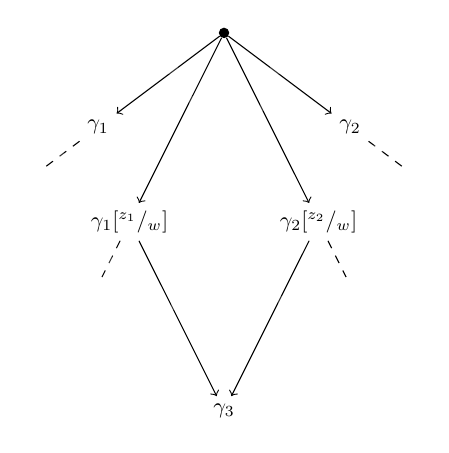
\begin{tikzpicture}[scale=0.8, transform shape]
					\tikzstyle{all nodes}=[inner sep=0pt,minimum size=0.2cm,circle,fill=black]
					\draw 
					node[circle,fill=black,scale=0.5](A)at(5.5,1){}
					node(B)at(3.5,-0.5){$\gamma_1$}              
					node(C)at(7.5,-0.5){$\gamma_2$} 
					node(D)at(8.5,-1.25){}
					node(E)at(2.5,-1.25){}
					node(F)at(4,-2){$\gamma_1[^{z_1}/_w]$}
					node(G)at(7,-2){$\gamma_2[^{z_2}/_w]$}
					node(H)at(5.5,-5){$\gamma_3$}
					node(I)at(3.5,-3){}
					node(L)at(7.5,-3){};	
					
					\draw[->](A)--(C) node[pos=.4, fill=white, opacity=0.2, text opacity=1,right] {};%{$\Delta_1$};
					\draw[->](A)--(B) node[pos=.4, fill=white, opacity=0.2, text opacity=1,left] {};%{$\Delta_1$};	
					\draw[dashed,-](B)--(E) node[pos=.4, fill=white, opacity=0.2, text opacity=1,left] {};
					\draw[dashed,-](C)--(D) node[pos=.4, fill=white, opacity=0.2, text opacity=1,left] {};
					\draw[->](A)--(F) node[pos=.4, fill=white, opacity=0.2, text opacity=1,right] {};
					\draw[->](A)--(G) node[pos=.4, fill=white, opacity=0.2, text opacity=1,right] {};
					\draw[->](F)--(H) node[pos=.4, fill=white, opacity=0.2, text opacity=1,right] {};
					\draw[->](G)--(H) node[pos=.4, fill=white, opacity=0.2, text opacity=1,right] {};
					\draw[dashed,-](F)--(I) node[pos=.4, fill=white, opacity=0.2, text opacity=1,left] {};
					\draw[dashed,-](G)--(L) node[pos=.4, fill=white, opacity=0.2, text opacity=1,left] {};
				\end{tikzpicture}
				\vfil
			}
			\caption{Proposition~\ref{lemma:upto} (item 2), Lemma~\ref{mono}, and the restriction to fair computations ensure confluence.}
			\label{fig:conf2}
		\end{minipage}
		\hfil
		
	\end{figure}
	
	
	


Thus, fair computations originating from a configuration are either all finite or all infinite, 
and furthermore  they have the same result.
 
%\subsection{Observational Semantics}
Now, let us denote by $\mathit{Result}(\gamma)$ the result of a configuration 
$\gamma$, which is obtained as the result of any fair computation originating from it.
%
 We are now ready to propose our first semantics.

\begin{definition}[Observational equivalence]\label{def:obequivalence}
Let $A, B \in \mathcal {A}$ be agents. We say that they are observationally equivalent  and we write 
$A \sim_o B$ if 
$\mathit{Result}(\langle A, \sigma \rangle) = \mathit{Result}(\langle B, \sigma \rangle)$
for all $\sigma \in  \C^\otimes$.
%Let $\mathcal{O} : (\mathcal{A} \rrarrow \mathcal{C}^\otimes) \rrarrow \mathcal{C}$ be the function given by 
%$\mathcal{O}({A})(\sigma) = \mathit{Result}(\langle A, \sigma \rangle)$.
%We say that $A$ and $B$ are \emph{observationally equivalent} ($A \sim_o B$) if $\mathcal{O}(A) = \mathcal{O}(B)$.
\end{definition}

It is easy to show $ \sim_o$ to be preserved by all contexts, i.e., it is a \emph{congruence}.
%\footnote{Recall that a context $C[\bullet]$ is a syntactic expression with a single hole $\bullet$ 
%such that replacing $\bullet$ with an agent $A$ in the context produces an agent, denoted by $C[A]$.
% For example if $C[\bullet]$ is the context $\tell(c) \parallel \bullet$  then $C[A] =  \tell(c) \parallel A.$
 %An equivalence $\cong$ between agents is a congruence if $A \cong B$ implies $C[A] \cong C[B]$
  %for every context $C[\bullet].$}


\section{Saturated Bisimulation}\label{sec:saturated}
As proposed in \cite{pippo} for crisp languages, we define a barbed equivalence between two agents~\cite{barbed}.  
%
Intuitively, barbs are basic observations (predicates) on the states of a system, and in our case they correspond 
to the compact constraints in $\mathcal{C}^\otimes$.

\begin{definition} [Barbs]
Let $\langle A, \sigma \rangle$ be a configuration and $c \in \mathcal{C}^\otimes$
and we say that $\langle A, \sigma \rangle$ verifies $c$, or that $\langle A, \sigma \rangle \downarrow_c$ holds, if  $c \leq \sigma$.
\end{definition}

However, since \emph{barbed bisimilarity} is an equivalence already for CCP, along~\cite{pippo}
we propose the use of \emph{saturated bisimilarity}
%~\cite{barbedMontanari} has been proposed 
in order to obtain a congruence:
%
Definition~\ref{def:strongsb} and Definition~\ref{def:weaksb} respectively provide the strong and weak definition of saturated bisimilarity.
%We say that $\gamma = \langle P, \sigma\rangle$ satisfies the barb $c$, written $\gamma \downarrow_c$,
%iff $\gamma \longrightarrow \gamma'$ and $\gamma' \downarrow_c$.
%\marginpar{Are barbs compact?}

\begin{definition}[Saturated bisimilarity]\label{def:strongsb} A saturated bisimulation is a symmetric relation $R$ on configurations such that whenever
%$(\gamma_1,\gamma_2) \in R$ with $\gamma_1 = \langle A, \sigma \rangle$
%and $\gamma_2 = \langle B, \rho \rangle$
$( \langle A, \sigma \rangle,\langle B, \rho \rangle) \in R$
\begin{enumerate}
\item if $\langle A, \sigma \rangle \downarrow_c$ then $\langle B, \rho \rangle \downarrow_c$;
\item if $\langle A, \sigma \rangle \longrightarrow \gamma'_1$ then there is $\gamma'_2$ such that $\langle B, \rho \rangle \longrightarrow \gamma'_2$ and $(\gamma'_1, \gamma'_2) \in R$;
\item $(\langle A,\sigma \otimes d\rangle, \langle B,\rho \otimes d \rangle) \in R$ for  all $d \in \mathcal{C}^\otimes$.
\end{enumerate}
We say that $\gamma_1$ and $\gamma_2$ are  saturated bisimilar ($\gamma_1  \sim_{\mathit{s}} \gamma_2$) if there exists a  saturated  bisimulation $R$ such that $(\gamma_1 , \gamma_2 ) \in R$. We write $A \sim_{\mathit{s}} B$ if $\langle A, \bot\rangle \sim_{\mathit{s}} \langle B, \bot \rangle$.
\end{definition}

We now let $\longrightarrow^*$ denote the reflexive and transitive closure of $\longrightarrow$, restricted to increasing computations.

\begin{definition} [Weak barbs]
Let $\langle A, \sigma \rangle$ be a configuration and $c \in \mathcal{C}^\otimes$.
We say that $\langle A, \sigma \rangle$ weakly verifies $c$, or that $\langle A, \sigma \rangle \Downarrow_c$ holds, 
if  there exists $\gamma' = \langle B, \rho \rangle$ such that 
$\gamma \longrightarrow^* \gamma'$ and $c \leq \exists_{X} \rho$ for $X = fv(\gamma') \setminus fv(\gamma)$.
\end{definition}

\begin{definition}[Weak saturated bisimilarity]\label{def:weaksb} A weak saturated bisimulation is a symmetric relation $R$ on configurations such that whenever
%$(\gamma_1,\gamma_2) \in R$ with $\gamma_1 = \langle A, \sigma \rangle$
%and $\gamma_2 = \langle B, \rho \rangle$
$( \langle A, \sigma \rangle,\langle B, \rho \rangle) \in R$
\begin{enumerate}
\item if $\langle A, \sigma \rangle \downarrow_c$ then $\langle B, \rho \rangle \Downarrow_c$;
\item if $\langle A, \sigma \rangle \longrightarrow \gamma'_1$ then there is $\gamma'_2$ such that $\langle B, \rho \rangle \longrightarrow^* \gamma'_2$ and $(\gamma'_1, \gamma'_2) \in R$;
\item $(\langle A,\sigma \otimes d\rangle, \langle B,\rho \otimes d \rangle) \in R$ for  all $d \in \mathcal{C}^\otimes$.
\end{enumerate}
We say that $\gamma_1$ and $\gamma_2$ are  weakly saturated bisimilar ($\gamma_1  \approx_{\mathit{s}} \gamma_2$) if there exists a  
weak saturated  bisimulation $R$ such that $(\gamma_1 , \gamma_2 ) \in R$. 
We write $A \approx_{\mathit{s}} B$ if $\langle A, \bot\rangle \approx_{\mathit{s}} \langle B, \bot \rangle$.
\end{definition}

The asymmetry is functional to later sections. However, it is clearly equivalent to the standard symmetric version.

\begin{definition}[Weak saturated bisimilarity, 2]\label{def:weaksb2}
Weak saturated bisimilarity coincides with the relation 
obtained from Definition~\ref{def:strongsb} by replacing $\longrightarrow$ with $\longrightarrow^*$ and $\downarrow_c$ with $\Downarrow_c$.
\end{definition}

Since $\sim_{\mathit{s}}$ (and $\approx_{\mathit{s}}$) is a saturated bisimulation, it is clearly upward closed and it is also a congruence: indeed, a context can modify the behaviour of a configuration only by adding constraints to its store.
%\marginpar{to be proved for $\exists_x-$ (not needed for Prop.3)}

\medskip
We now show that $\approx_{\mathit{s}}$, as given in Definition~\ref{def:weaksb}, coincides with the observational equivalence $\sim_o$ (see Definition~\ref{def:obequivalence}). First we recall the notion of and a classic result on \emph{cofinality}: two (possibly infinite) chains $c_0 \leq c_1 \leq \dots$ and  $d_0 \leq d_1 \leq \dots$ are said to be \emph{cofinal} if for all $c_i$ there exists a $d_j$ such that $c_i \leq d_j$ and, vice-versa, for all $d_i$ there exists a $c_j$ such that $d_i \leq c_j$.

\begin{lemma}\label{lem:cofinality} 
Let $c_0 \leq c_1 \leq \dots$ and $d_0 \leq d_1 \leq \dots $ be two chains. \emph{(1)} If they are cofinal, then they have the same limit, i.e., $\bigvee_i c_i = \bigvee_i d_i$. \emph{(2)} If the elements of the chains are $\otimes$-compact and $\bigvee_i c_i = \bigvee_i d_i$, then the two chains are cofinal.\end{lemma}
%\marginpar{questo richiede che tell inserisca solo compatti}
\begin{proof}
%[of Lemma~\ref{lem:cofinality}]
Let us tackle $(2)$, and consider the sequence $e_0 = c_0$ and $e_{i} = c_{i+1} \odiv c_i$.
Each $e_i$ is the difference between two consecutive elements of a chain.
%
Since the CLIM is invertible we have $c_k =  \bigotimes_{i \leq k} e_i$ and thus
$\bigvee_i c_i = \bigotimes_i e_i$. Since each $d_j$ is $\otimes$-compact and
$d_j \leq \bigotimes_i e_i$, there is a $k$ such that $d_j \leq \bigotimes_{i \leq k} e_i$.
The same reasoning is applied to the chain $d_0 \leq d_1 \leq \dots $, thus
the result holds.
\end{proof}


To prove Theorem~\ref{prop:weaksbequivobs}, besides cofinality from Lemma~\ref{lem:cofinality} we need to relate weak barbs and fair computations.

\begin{lemma}\label{lem:barbsfair}
Let $\xi = \gamma_0 \longrightarrow \gamma_1 \longrightarrow \ldots$ be a (possibly infinite) fair computation. If $\gamma_0 \Downarrow_d$ then there exists a store $\sigma_i$ in $\xi$ such that $d \leq \exists_{X_i} \sigma_i$ for $X_i = fv(\gamma_i) \setminus fv(\gamma_0)$.
\end{lemma}

The lemma is a direct consequence of confluence (see Theorem~\ref{prop:confluence}).

\begin{theorem}\label{prop:weaksbequivobs}
Let $A$, $B$ be agents. Then $A \sim_o B$ if and only if $A \approx_{\mathit{s}} B$.
\end{theorem}
%\marginpar{L'unica cosa da provare \`e in realt\`a il Lemma 1}
\begin{proof}%[of Proposition~\ref{prop:weaksbequivobs}]
	The proof proceeds as follows.
	\begin{description}
		\item[From $\approx_{\mathit{s}}$ to $\sim_o$.] Assume  $\langle A, \bot \rangle \approx_{\mathit{s}} \langle B, \bot \rangle$ and take a $\otimes$-compact $c \in \mathcal{C}^\otimes$. Let
		\begin{equation}\label{comp:1}\langle A, c \rangle \longrightarrow \langle A_0, \sigma_0 \rangle \longrightarrow \langle A_1, \sigma_1 \rangle \longrightarrow \dots \longrightarrow \langle A_n, \sigma_n \rangle \dots \longrightarrow \dots
		\end{equation}
		\begin{equation}\label{comp:2}\langle B, c \rangle \longrightarrow \langle B_0, \rho_0 \rangle \longrightarrow \langle B_1, \rho_1 \rangle \longrightarrow \dots \longrightarrow \langle B_n, \rho_n \rangle \dots \longrightarrow \dots
		\end{equation}
		
		be two fair computations. Since $\approx_{\mathit{s}}$ is upward closed, 
		$\langle A, c \rangle \approx_{\mathit{s}} \langle B, c \rangle$ and thus $\langle B, c\rangle \Downarrow_{\sigma_i}$ for all $\sigma_i$. By Lemma~\ref{lem:barbsfair}, it follows that there exists an $\rho_j$ (in the above computation) such that 
		$\exists_{\Gamma_i} \sigma_i \leq \sigma_i \leq \exists_{\Gamma'_j} \rho_j$, and analogously for all $\rho_i$.
		%there exists a $\sigma_j$ such that $\rho_i \leq \sigma_j$. 
		Then $\sigma_0 \leq \sigma_1 \leq \dots$  and $\rho_0 \leq \rho_1 \leq \dots$ are cofinal and by Lemma~\ref{lem:cofinality} it holds that $\bigvee_i \exists_{\Gamma_i} \sigma_i = \bigvee_i \exists_{\Gamma'_i} \rho_i$, which means 
		$\mathit{Result}(\langle A, c \rangle) = \mathit{Result}(\langle B, c \rangle)$.
		%\marginpar{before it was $\bigvee_i \Gamma_i \sigma_i$, no $\exists$}
		
		\item[From $\sim_o$ to $\approx_{\mathit{s}}$.] Assume $A \sim_o B$. First, we show that $\langle A, c\rangle$ and $\langle B, c\rangle$ satisfy the same weak barbs  for all $c \in \mathcal{C}$. Let (\ref{comp:1}) and (\ref{comp:2}) be two fair computations. Since $A \sim_o B$, then $\bigvee_i \exists_{\Gamma_i} \sigma_i = \bigvee_i \exists_{\Gamma'_j} \rho_i$. Since all (the projections of) the intermediate stores of the computations are $\otimes$-compact,
		%(by Lemma~\ref{comp}),
		%\marginpar{da rivedere la sintassi per la tell}
		then by Lemma~\ref{lem:cofinality} for all $\sigma_i$ there exists an $\rho_j$ such that $\exists_{\Gamma_i} \sigma_i \leq \exists_{\Gamma'_j} \rho_j$. 
		Now suppose that $\langle A, c \rangle \Downarrow_d$. By Lemma~\ref{lem:barbsfair}, 
		there exists a $\sigma_i$ 
		%(in the above computation) 
		such that $d \leq \exists_{\Gamma_i} \sigma_i$. Thus 
		%$d \leq \exists_{\Gamma_i} \sigma_i \leq \exists_{\Gamma_i} \rho_j$ that means 
		$\langle B, c\rangle \Downarrow_d$.
		
		It is now easy to prove that
		$R = \{(\gamma_1, \gamma_2) \mid \exists c. \langle A, c \rangle \longrightarrow^* \gamma_1 \& \langle B, c\rangle \longrightarrow^* \gamma_2\}$
		is a weak saturated bisimulation (Definition~\ref{def:weaksb}). Take $(\gamma_1 , \gamma_2 ) \in R$.
		If $\gamma_1 \Downarrow_d$ then $\langle A, c\rangle \Downarrow_d$ and, by the above observation, $\langle B, c\rangle \Downarrow_d$. Since \SCCP is
		confluent, also $\gamma_2 \Downarrow_d$.
		The fact that R is closed under $\longrightarrow^*$ is evident from the definition of $R$. While
		for proving that R is upward-closed take $\gamma_1 = \langle A', \sigma'\rangle$ and $\gamma_2 = \langle B', \rho'\rangle$. By item 4 of Lemma~\ref{mono} (i.e., language monotonicity)
		for all $a \in \mathcal{C}, \langle A, c \otimes a\rangle \longrightarrow^* \langle A', \sigma' \otimes a \rangle$ and $\langle B, c \otimes a\rangle \longrightarrow^* \langle B', \rho'  \otimes a \rangle$. Thus, by definition of $R$, $(\langle A',\sigma' \otimes a \rangle, \langle B',\rho' \otimes a\rangle) \in R$.
	\end{description} 
\end{proof}
\end{document}